\section{TỨ GIÁC NỘI TIẾP}
\subsubsection{Kiến thức trọng tâm}
\begin{tomtat}
	\begin{dn}
		\immini{
			\begin{itemize}
				\item Một tứ giác có bốn đỉnh nằm trên một đường tròn được gọi là \textit{tứ giác nội tiếp đường tròn} (gọi tắt là \textit{tứ giác nội tiếp}).
				\item Đường tròn đi qua bốn đỉnh của tứ giác gọi là \textit{đường tròn ngoại tiếp} tứ giác đó.
			\end{itemize}
		}{
			\begin{tikzpicture}[>=stealth,line join=round,line cap=round,font=\footnotesize,scale=1]
				\path
				(0,0) coordinate (O)
				($(O) + (-15:1.7)$) coordinate (A)
				($(O) + (50:1.7)$) coordinate (B)
				($(O) + (120:1.7)$) coordinate (C)
				($(O) + (210:1.7)$) coordinate (D)
				;
				\draw (O) circle (1.7 cm);
				\draw (A)--(B)--(C)--(D)--cycle;
				\foreach \x in {O,A,B,C,D} \fill[black] (\x) circle (1pt);
			\end{tikzpicture}
		}
	\end{dn}
	
	\begin{dl}%[Dự án EX-9-Đề Cương Toán 9]%[NGOCTRUNG]%[9H9N2-1]
		Trong một tứ giác nội tiếp, tổng số đo hai góc đối nhau bằng $180^\circ$.
	\end{dl}
	
	\begin{dl}%[Dự án EX-9-Đề Cương Toán 9]%[NGOCTRUNG]%[9H9N2-1]
		\begin{itemize}
			\item	Hình chữ nhật, hình vuông là các tứ giác nội tiếp.
			\item Đường tròn ngoại tiếp hình chữ nhật, hình vuông có tâm là giao điểm của hai đường chéo và có bán kính bằng nửa đường chéo.
		\end{itemize}
		\begin{center}
			\begin{tikzpicture}[scale=0.7, font=\footnotesize, line join=round, line cap=round, >=stealth]
				\coordinate (O) at (-2,3);
				\coordinate (A) at (-4.54,4.6);
				\coordinate (B) at (0.54,4.59);
				\coordinate (C) at (0.54,1.4);
				\coordinate (D) at (-4.54,1.41);
				\draw (A)--(O)--(B) (D)--(O);
				\draw[name path=circ1] (O) circle (3);
				\draw (D)  node[left]{$D$}--(A) node[left]{$A$}--(B) node[right]{$B$}--(C) node[right]{$C$}--(D);
				\draw (O)  node[above]{$O$}--(C);
				
				% Chấm các điểm 
				\filldraw (A) circle (1.5pt);
				\filldraw (B) circle (1.5pt);
				\filldraw (C) circle (1.5pt);
				\filldraw (D) circle (1.5pt);
				\filldraw (O) circle (1.5pt);
				
				\coordinate (I) at (5,3);
				\coordinate (Q) at (2.75,1.01);
				\coordinate (M) at (2.77,5.01);
				\coordinate (N) at (7.25,4.99);
				\coordinate (P) at (7.23,0.99);
				\draw (N)--(I)--(M) (Q)--(I);
				\draw[name path=circ1] (I) circle (3);
				\draw (Q)  node[left]{$Q$}--(M) node[left]{$M$}--(N) node[right]{$N$}--(P) node[right]{$P$}--(Q);
				\draw (I)  node[above]{$I$}--(P);
				\path (Q)--(M)node[midway, left]{$a$};
				
				% Chấm các điểm 
				\filldraw (Q) circle (1.5pt);
				\filldraw (M) circle (1.5pt);
				\filldraw (N) circle (1.5pt);
				\filldraw (P) circle (1.5pt);
				\filldraw (I) circle (1.5pt);
			\end{tikzpicture}
		\end{center}
	\end{dl}
	\begin{note}
		Bán kính đường tròn ngoại tiếp hình vuông cạnh $a$ bằng $\dfrac{a\sqrt{2}}{2}$. 
	\end{note}
\end{tomtat}

\subsubsection{Bài tập}

\begin{dang}{Nhận diện tứ giác nội tiếp và tính toán các yếu tố liên quan đến tứ giác nội tiếp}
	\begin{itemize}
		\item Một tứ giác có bốn đỉnh nằm trên một đường tròn được gọi là \textit{tứ giác nội tiếp đường tròn} (gọi tắt là \textit{tứ giác nội tiếp}). \textbf{Đặc biệt}, hình chữ nhật và hình vuông là các tứ giác nội tiếp đường tròn có tâm là giao điểm của hai đường chéo.
		\item Đường tròn đi qua bốn đỉnh của tứ giác gọi là \textit{đường tròn ngoại tiếp} tứ giác đó.
		\item Trong một tứ giác nội tiếp, tổng số đo hai góc đối nhau bằng $180^\circ$.
	\end{itemize}
\end{dang}

\begin{vd}%[SGK CTST Toán 9]%[Dự án EX-9-Đề Cương Toán 9]%[NGOCTRUNG]%[9H3N2-1]
	Tìm tứ giác nội tiếp trong các hình sau
	\begin{center}
		\begin{tikzpicture}[scale=0.5, font=\footnotesize, line join=round, line cap=round, >=stealth]
			\coordinate (O) at (0,0);
			\coordinate (A) at (-1.01,2.83);
			\coordinate (B) at (-2.98,0.32);
			\coordinate (C) at (-2.02,-2.22);
			\coordinate (D) at (2.83,-1);
			\draw (A)--(B)--(C)--(D)--(A);
			\draw[name path=circ1] (O) circle (3);
			\node at (0,-3.5) {a)};
			% Chấm điểm
			\filldraw (A) circle (1.5pt);
			\filldraw (B) circle (1.5pt);
			\filldraw (C) circle (1.5pt);
			\filldraw (D) circle (1.5pt);
			\filldraw (O) circle (1.5pt);
		\end{tikzpicture}	
		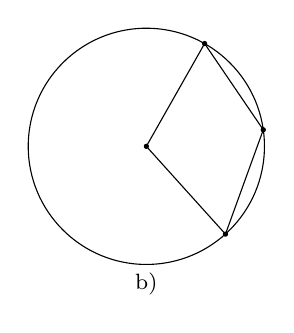
\begin{tikzpicture}[scale=0.5, font=\footnotesize, line join=round, line cap=round, >=stealth]
			\coordinate (G) at (3,0);
			\coordinate (I) at (4.48,2.61);
			\coordinate (J) at (5.97,0.42);
			\coordinate (K) at (5.01,-2.23);
			\draw (G)--(I)--(J)--(K)--(G);
			\draw (G) circle (3);
			\node at (3,-3.5) {b)};
			% Chấm điểm
			\filldraw (G) circle (1.5pt);
			\filldraw (I) circle (1.5pt);
			\filldraw (J) circle (1.5pt);
			\filldraw (K) circle (1.5pt);
		\end{tikzpicture}
		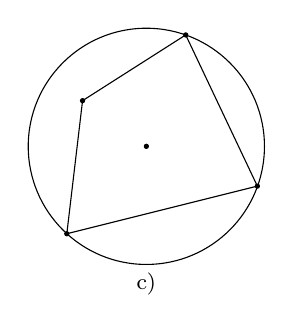
\begin{tikzpicture}[scale=0.5, font=\footnotesize, line join=round, line cap=round, >=stealth]
			\coordinate (G) at (6,0);
			\coordinate (I) at (7,2.83);
			\coordinate (J) at (4.38,1.16);
			\coordinate (K) at (3.98,-2.22);
			\coordinate (D) at (8.82,-1.01);
			\draw (I)--(J)--(K)--(D)--(I);
			\draw (G) circle (3);
			\node at (6,-3.5) {c)};
			% Chấm điểm
			\filldraw (G) circle (1.5pt);
			\filldraw (I) circle (1.5pt);
			\filldraw (J) circle (1.5pt);
			\filldraw (K) circle (1.5pt);
			\filldraw (D) circle (1.5pt);
		\end{tikzpicture}
		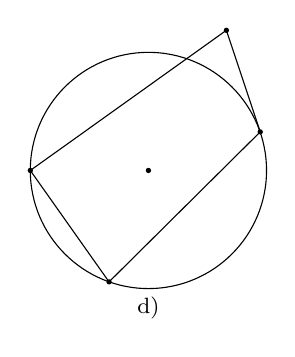
\begin{tikzpicture}[scale=0.5, font=\footnotesize, line join=round, line cap=round, >=stealth]
			\coordinate (G) at (9,0);
			\coordinate (I) at (10.98,3.56);
			\coordinate (J) at (6,0);
			\coordinate (K) at (8,-2.83);
			\coordinate (D) at (11.84,0.98);
			\draw (I)--(J)--(K)--(D)--(I);
			\draw (G) circle (3);
			\node at (9,-3.5) {d)};
			% Chấm điểm
			\filldraw (G) circle (1.5pt);
			\filldraw (I) circle (1.5pt);
			\filldraw (J) circle (1.5pt);
			\filldraw (K) circle (1.5pt);
			\filldraw (D) circle (1.5pt);
		\end{tikzpicture}
	\end{center}
	\loigiai{
		Tứ giác trong hình a có bốn đỉnh đều nằm trên đường tròn nên là tứ giác nội tiếp. Còn các tứ giác trong hình còn lại không phải là tứ giác nội tiếp.
	}
\end{vd}

\begin{vd}%[SGK CTST Toán 9]%[Dự án EX-9-Đề Cương Toán 9]%[NGOCTRUNG]%[9H3N2-2]
	Tìm $x$ và $y$ của tứ giác có trong hình bên dưới.
	\begin{center}
		\begin{tikzpicture}[scale=0.75, font=\footnotesize, line join=round, line cap=round, >=stealth]
			\coordinate (O) at (6,2);
			\coordinate (A) at (6,5);
			\coordinate (B) at (3,2);
			\coordinate (C) at (8.82,0.97);
			\coordinate (D) at (8.24,4);
			\draw (A)--(B)--(C)--(D)--(A);
			\draw[name path=circ1] (O) circle (3);
			\draw pic[double,draw=black, angle eccentricity=1.5, angle radius=.3cm, color=red]
			{angle=A--D--C};
			\pic[draw,angle radius=0.3cm] {angle = C--B--A};
			\pic[draw,angle radius=0.3cm,color=blue] {angle = B--A--D};
			\draw pic[draw=black, angle eccentricity=1.5, angle radius=.3cm, color=red]
			{angle=D--C--B};
			\draw (D) circle (1pt)+(220:7mm)node{$y$};
			\draw (C) circle (1pt)+(140:7mm)node{$x$};
			\draw (B) circle (1pt)+(10:10mm)node{$63^\circ$};
			\draw (A) circle (1pt)+(-70:7mm)node{$104^\circ$};
		\end{tikzpicture}
	\end{center}
	\loigiai{
		Tứ giác trong hình đã cho là tứ giác nội tiếp.\\
		Do đó 
		\begin{itemize}
			\item $x+104^\circ=180^\circ$, suy ra $x=180^\circ-104^\circ=76^\circ$.
			\item $y+63^\circ=180^\circ$, suy ra $y=180^\circ-63^\circ=117^\circ$.
		\end{itemize}
	}
\end{vd}

\begin{vd}%[SGK CTST Toán 9]%[Dự án EX-9-Đề Cương Toán 9]%[NGOCTRUNG]%[9H3N2-2]
	Tìm số đo các góc chưa biết của tứ giác $ABCD$ trong hình bên dưới.
	\begin{center}
		\begin{tikzpicture}[scale=0.75, font=\footnotesize, line join=round, line cap=round, >=stealth]
			\coordinate (O) at (5,5);
			\coordinate (A) at (3.01,7.25);
			\coordinate (B) at (7.82,3.98);
			\coordinate (C) at (3.99,2.17);
			\coordinate (D) at (2.17,4);
			\draw (A)node[above left]{$A$}--(B)node[below right]{$B$}--(C)node[below left]{$C$}--(D)node[below left]{$D$}--(A);
			\draw pic[double,draw=black, angle eccentricity=2, angle radius=.4cm, color=blue]
			{angle=A--B--C}; 
			\draw pic[draw=black, angle eccentricity=2, angle radius=.3cm, color=blue]
			{angle=B--C--D}; 
			\draw[name path=circ1] (O) circle (3);
			\draw (B) circle (1pt)+(177:9.5mm)node{$57^\circ$};
			\draw (C) circle (1pt)+(80:7mm)node{$93^\circ$};
			% Chấm điểm
			\filldraw (A) circle (1pt);
			\filldraw (D) circle (1pt);
			\filldraw (O) circle (1pt);
		\end{tikzpicture}
	\end{center}
	\loigiai{
		Tứ giác $ABCD$ trong hình đã cho là tứ giác nội tiếp.\\
		Do đó
		\begin{itemize}
			\item $\widehat{A}+\widehat{C}=180^\circ$, suy ra $\widehat{C}=180^\circ-\widehat{A}=180^\circ-93^\circ=87^\circ$.
			\item $\widehat{B}+\widehat{D}=180^\circ$, suy ra $\widehat{D}=180^\circ-\widehat{B}=180^\circ-57^\circ=123^\circ$.
		\end{itemize}
	}
\end{vd}

\begin{vd}%[SGK CTST Toán 9]%[Dự án EX-9-Đề Cương Toán 9]%[NGOCTRUNG]%[9H3H2-3]
	Xác định tâm và tính bán kính đường tròn ngoại tiếp hình chữ nhật và hình vuông trong hình bên dưới.
	\begin{center}
		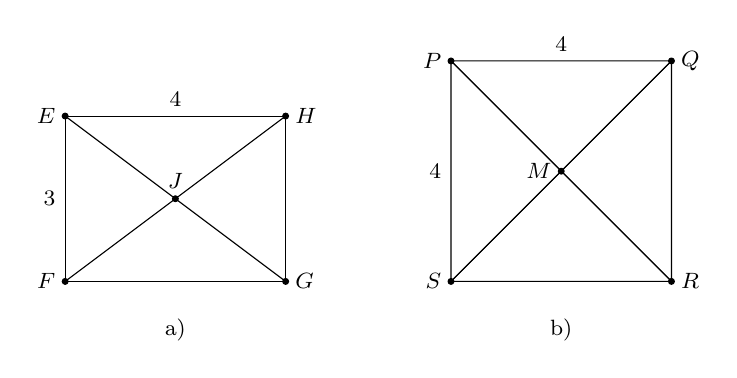
\begin{tikzpicture}[scale=0.7, font=\footnotesize, line join=round, line cap=round, >=stealth]
			\coordinate (J) at (3,5/2);
			\coordinate (E) at (1,4);
			\coordinate (F) at (1,1);
			\coordinate (G) at (5,1);
			\coordinate (H) at (5,4);
			\draw (J)--(F) (E)--(J) (H)--(J);
			\draw (E)  node[left]{$E$}--(F) node[left]{$F$}--(G) node[right]{$G$}--(H) node[right]{$H$}--(E);
			\draw (J)  node[above]{$J$}--(G);
			\path (F)--(E)node[midway, left]{$3$};
			\path (E)--(H)node[midway, sloped, above]{$4$};
			% Chấm điểm phần 1
			\filldraw (E) circle (1.5pt);
			\filldraw (F) circle (1.5pt);
			\filldraw (G) circle (1.5pt);
			\filldraw (H) circle (1.5pt);
			\filldraw (J) circle (1.5pt);
			\coordinate (M) at (10,3);
			\coordinate (S) at (8,1);
			\coordinate (P) at (8,5);
			\coordinate (Q) at (12,5);
			\coordinate (R) at (12,1);
			\draw (M)--(S) (P)--(M) (Q)--(M)(P)--(Q) (S)--(R);
			\draw (S)  node[left]{$S$}--(P) node[left]{$P$}--(R) node[right]{$R$}--(Q) node[right]{$Q$}--(S);
			\draw (M)  node[left]{$M$}--(R);
			\path (S)--(P)node[midway, left]{$4$};
			\path (P)--(Q)node[midway, sloped, above]{$4$};
			% Chấm điểm phần 2
			\filldraw (S) circle (1.5pt);
			\filldraw (P) circle (1.5pt);
			\filldraw (Q) circle (1.5pt);
			\filldraw (R) circle (1.5pt);
			\filldraw (M) circle (1.5pt);
			\fill (3,0.5) node[below]{a)};
			\fill (10,0.5) node[below]{b)};
		\end{tikzpicture}
	\end{center}
	\loigiai{
		Hình chữ nhật $EFGH$ có $J$ là giao điểm của hai đường chéo.\\
		Xét $\triangle EFH$ vuông tại $E$, áp dụng định lí Pythagore, ta có  $$FH=\sqrt{EF^2+EH^2}=\sqrt{3^2+4^2}=5.$$
		Suy ra đường tròn ngoại tiếp hình chữ nhật $EFGH$ có tâm $J$ và bán kính $R=\dfrac{EF}{2}=\dfrac{5}{2}$.\\
		Hình vuông $PQRS$ có $M$ là giao điểm của hai đường chéo.\\
		Xét $\triangle PRQ$ vuông tại $Q$, áp dụng định lí Pythagore, ta có
		$$PR=\sqrt{PQ^2+QR^2}=\sqrt{4^2+4^2}=4\sqrt{2}.$$
		Suy ra đường tròn ngoại tiếp hình vuông $PQRS$ có tâm $M$ và bán kính $R=\dfrac{PR}{2}=2\sqrt{2}$.
	}
\end{vd}

\begin{bt}%[SGK KNTT Toán 9]%[9H3N2-1]
	Trong các hình sau, hình nào vẽ một tứ giác nội tiếp một đường tròn?
	\begin{center}
		\begin{tabular}{ccc}
			\begin{tikzpicture}[>=stealth,line join=round,line cap=round,font=\footnotesize,scale=0.5]
				\coordinate (O) at (0,0);
				\coordinate (A) at (-1.01,2.83);
				\coordinate (B) at (-2.98,0.32);
				\coordinate (C) at (-2.02,-2.22);
				\coordinate (D) at (2.83,-1);
				\draw (A)--(B)--(C)--(D)--(A);
				\draw[name path=circ1] (O) circle (3);
			\end{tikzpicture}
			&
			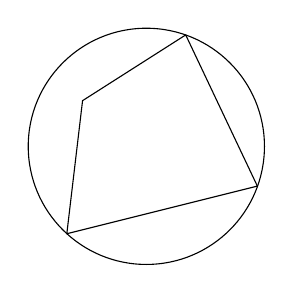
\begin{tikzpicture}[>=stealth,line join=round,line cap=round,font=\footnotesize,scale=0.5]
				\coordinate (G) at (6,0);
				\coordinate (I) at (7,2.83);
				\coordinate (J) at (4.38,1.16);
				\coordinate (K) at (3.98,-2.22);
				\coordinate (D) at (8.82,-1.01);
				\draw (I)--(J)--(K)--(D)--(I);
				\draw (G) circle (3);
			\end{tikzpicture}
			&
			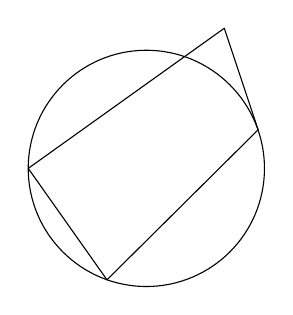
\begin{tikzpicture}[>=stealth,line join=round,line cap=round,font=\footnotesize,scale=0.5]
				\coordinate (G) at (9,0);
				\coordinate (I) at (10.98,3.56);
				\coordinate (J) at (6,0);
				\coordinate (K) at (8,-2.83);
				\coordinate (D) at (11.84,0.98);
				\draw (I)--(J)--(K)--(D)--(I);
				\draw (G) circle (3);
			\end{tikzpicture}
			\\a)&b)&c)
		\end{tabular}
	\end{center}
	\loigiai{
		Tứ giác trong a) có bốn đỉnh đều nằm trên đường tròn nên là tứ giác nội tiếp. Còn các tứ giác trong hình còn lại không phải là tứ giác nội tiếp vì có ba đỉnh nằm trên đường tròn và đỉnh còn lại không nằm trên đường tròn.
	}
\end{bt}

\begin{bt}%[SGK CD Toán 9]%[9H3N2-1]
	Trong các hình a), b), ở hình nào ta có tứ giác $ABCD$ 
	nội tiếp đường tròn $(O)$? Vì sao?
	\begin{center}
		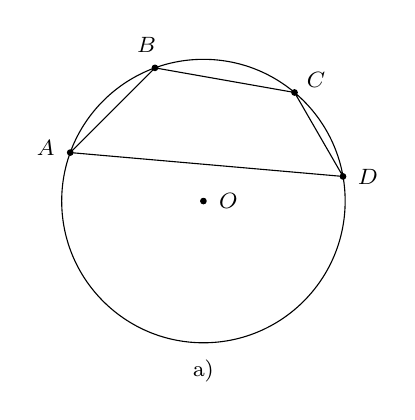
\begin{tikzpicture}[scale=1, font=\footnotesize, line 
			join=round, line 
			cap=round, >=stealth]
			\def\r{1.8}
			\path (0,0) coordinate (O)
			(160:\r) coordinate (A)
			(110:\r) coordinate (B)
			(10:\r) coordinate (D)
			(50:\r) coordinate (C)
			(-90:\r*1.2) coordinate (E) node {a)}
			;
			\draw (O) circle (\r) (A)--(B)--(C)--(D)--cycle
			;
			\foreach \d/\g in {A/170, B/110, C/30,D/0,O/0}	
			\path[draw,fill=black] (\d) circle(1pt) + (\g:9pt) node 
			{$\d$};
		\end{tikzpicture}\hspace*{1cm}
		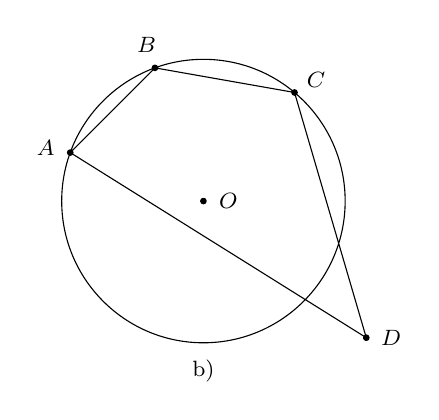
\begin{tikzpicture}[scale=1, font=\footnotesize, line 
			join=round, line 
			cap=round, >=stealth]
			\def\r{1.8}
			\path (0,0) coordinate (O)
			(160:\r) coordinate (A)
			(110:\r) coordinate (B)
			(-40:\r*1.5) coordinate (D)
			(50:\r) coordinate (C)
			(-90:\r*1.2) coordinate (E) node {b)}
			;
			\draw (O) circle (\r) (A)--(B)--(C)--(D)--cycle
			;
			\foreach \d/\g in {A/170, B/110, C/30,D/0,O/0}	
			\path[draw,fill=black] (\d) circle(1pt) + (\g:9pt) node 
			{$\d$};
		\end{tikzpicture}
	\end{center}
	\loigiai{
		\begin{itemize}
			\item Ở Hình a), tứ giác $ABCD$ có bốn đỉnh đều nằm trên đường tròn $(O)$ do đó tứ giác $ABCD$ nội tiếp $(O)$.
			\item Ở Hình b), tứ giác $ABCD$ chỉ có ba đỉnh $A$, $B$, $C$ nằm trên đường tròn $(O)$ do đó tứ giác $ABCD$ không nội tiếp $(O)$.
		\end{itemize}
	}
\end{bt}

\begin{bt}%[SGK CD Toán 9]%[9H3N2-1]
	\immini{
		Quan sát hình bên và cho biết trong hai đường tròn $(O)$ và $(I)$, đường tròn nào ngoại tiếp tứ giác $ABCD$, đường tròn nào ngoại tiếp tứ giác $ABMN$.
	}{
		\begin{tikzpicture}[scale=0.7, font=\footnotesize, line 
			join=round, line cap=round, >=stealth]
			\def\r{3}
			\def\gocA{120}
			\path (0,0) coordinate (O)
			(\gocA:\r) coordinate (D)
			(25:\r) coordinate (A)
			(210:\r) coordinate (C)
			(-30:\r) coordinate (B)
			($(C)!1.8!(B)$) coordinate (M)
			($(B)!.5!(M)$) coordinate (M')
			($(M')!1!-90:(B)$) coordinate (x)
			($(B)!(O)!(A)$) coordinate (H)
			(intersection of O--H and M'--x) coordinate (I)
			($(A)+(10:\r*0.5)$) coordinate (Ax)
			($(Ax)!(I)!(A)$) coordinate (I')
			($(A)!2!(I')$) coordinate (N)
			($(B)+(-90:\r*0.7)$) coordinate (E) node {Hình $28$}
			;
			\draw[red] (I) let \p1 = ($(I)-(A)$) in circle 
			({veclen(\x1,\y1)});
			\draw [blue] (O) circle (\r);
			\draw  (A)--(B)--(C)--(D)--cycle (B)--(M)--(N)--(A)
			;
			\foreach \d/\g in {A/80, B/-90, 
				C/230,D/130,O/0,I/0,M/-45,N/70}	
			\path[draw,fill=white] (\d) circle(1pt) + (\g:13pt) node 
			{$\d$};
	\end{tikzpicture}}
	\loigiai{
		\begin{itemize}
			\item Đường tròn $(O)$ ngoại tiếp tứ giác $ABCD$.
			\item Đường tròn $(I)$ ngoại tiếp tứ giác $ABMN$. 
		\end{itemize}
	}
\end{bt}

\begin{bt}%[SGK CTST Toán 9]%[9H3H2-2]
	Cho $ABCD$ là tứ giác nội tiếp. Hãy hoàn thành các giá trị còn thiếu của bảng sau vào vở.
	\begin{center}
		\begin{tabular}{|c|c|c|c|c|}
			\hline
			\diagbox{Góc}{Trường hợp}	& \textbf{$1$} & \textbf{$2$} & \textbf{$3$} & \textbf{$4$} \\
			\hline
			$\widehat{A}$	& $90^\circ$ &  ?  &  ?  & $66^\circ$ \\
			\hline
			$\widehat{B}$	& $120^\circ$ & ?   & $75^\circ$ &  ?  \\
			\hline
			$\widehat{C}$	& ? & $80^\circ$ & $89^\circ$ &  ?  \\
			\hline
			$\widehat{D}$	& ?  & $70^\circ$ &  ?  & $88^\circ$ \\
			\hline
		\end{tabular}
	\end{center}
	\loigiai{
		\begin{center}
			\begin{tabular}{|c|c|c|c|c|}
				\hline
				\diagbox{Góc}{Trường hợp}	& \textbf{$1$} & \textbf{$2$} & \textbf{$3$} & \textbf{$4$} \\
				\hline
				$\widehat{A}$	& $90^\circ$ &  $100^\circ$ &  $91^\circ$ & $66^\circ$ \\
				\hline
				$\widehat{B}$	& $120^\circ$ & $110^\circ$  & $75^\circ$ &  $92^\circ$ \\
				\hline
				$\widehat{C}$	& $90^\circ$ & $80^\circ$ & $89^\circ$ &  $114^\circ$ \\
				\hline
				$\widehat{D}$	& $60^\circ$ & $70^\circ$ &  $105^\circ$ & $88^\circ$ \\
				\hline
			\end{tabular}
		\end{center}
	}
\end{bt}

\begin{bt}%[SGK CD Toán 9]%[9H3H2-2]
	Cho tứ giác $ABCD$ nội tiếp đường tròn. Tính số đo các góc còn 
	lại của tứ giác đó trong mỗi trường hợp sau
	\begin{multicols}{2}
		\begin{enumerate}
			\item $\widehat{A}=60^{\circ}$ và $\widehat{B}=125^{\circ}$;
			\item $\widehat{B}=95^{\circ}$ và $\widehat{C}=67^{\circ}$;
			\item $\widehat{C}=75^{\circ}$ và $\widehat{D}=115^{\circ}$;
			\item $\widehat{D}=103^{\circ}$ và $\widehat{A}=117^{\circ}$.
		\end{enumerate}
	\end{multicols}
	\loigiai{
		\begin{enumerate}
			\item Vì tứ giác $ABCD$ nội tiếp đường tròn, do đó
			\begin{itemize}
				\item $\widehat{A}+\widehat{C}=180^\circ$ suy ra $\widehat{C} = 180^\circ - \widehat{A} = 180^\circ - 60^\circ = 120^\circ$.
				\item $\widehat{B}+\widehat{D}=180^\circ$ suy ra $
				\widehat{D} = 180^\circ - \widehat{B} = 180^\circ - 125^\circ = 55^\circ$.
			\end{itemize}
			\item Vì tứ giác $ABCD$ nội tiếp đường tròn, do đó
			\begin{itemize}
				\item $\widehat{B}+\widehat{D}=180^\circ$ suy ra $
				\widehat{D} = 180^\circ - \widehat{B} = 180^\circ - 95^\circ = 85^\circ$.
				\item $\widehat{A}+\widehat{C}=180^\circ$ suy ra $\widehat{A} = 180^\circ - \widehat{C}
				= 180^\circ - 67^\circ = 113^\circ$.
			\end{itemize}
			\item Vì tứ giác $ABCD$ nội tiếp đường tròn, do đó
			\begin{itemize}
				\item $\widehat{A}+\widehat{C}=180^\circ$ suy ra $
				\widehat{A} = 180^\circ - \widehat{C} = 180^\circ - 75^\circ = 105^\circ$.
				\item $\widehat{B}+\widehat{D}=180^\circ$ suy ra $\widehat{B} = 180^\circ - \widehat{D} = 180^\circ - 115^\circ = 65^\circ$.
			\end{itemize}
			\item Vì tứ giác $ABCD$ nội tiếp đường tròn, do đó
			\begin{itemize}
				\item $\widehat{B}+\widehat{D}=180^\circ$ suy ra $\widehat{B} = 180^\circ - \widehat{D} = 180^\circ - 103^\circ = 77^\circ$.
				\item $\widehat{A}+\widehat{C}=180^\circ$ suy ra $
				\widehat{C} = 180^\circ - \widehat{A} = 180^\circ - 117^\circ = 63^\circ$.
			\end{itemize}
		\end{enumerate}
	}
\end{bt}

\begin{bt}%[SGK CD Toán 9]%[9H3H2-2]
	Cho tam giác $ABC$ nội tiếp đường tròn $(O)$ thoả mãn 
	$\widehat{ABC}=60^{\circ}$, $\widehat{ACB}=70^{\circ}$. Giả sử 
	$D$ là điểm thuộc cung $BC$ không chứa $A$. Tính số đo góc $BDC$.
	\loigiai{
		\immini{
			Xét $\triangle ABC$, ta có
			\allowdisplaybreaks
			\begin{eqnarray*}
				\widehat{BAC}+\widehat{ABC}+\widehat{ACB}&=&180^\circ\\
				\widehat{BAC}+60^\circ+70^\circ&=&180^\circ\\
				\widehat{BAC}&=&50^\circ.
			\end{eqnarray*}
			Vì tứ giác $ABDC$ nội tiếp $(O)$ nên ta có
			\allowdisplaybreaks
			\begin{eqnarray*}
				\widehat{BAC}+\widehat{BDC}&=&180^\circ\\
				50^\circ+ \widehat{BDC}&=&180^\circ\\
				\widehat{BDC}&=&130^\circ.
			\end{eqnarray*}
			Vậy $\widehat{BDC} = 130^\circ$.
		}{
			\begin{tikzpicture}[scale=1, font=\footnotesize, line join=round, 
				line 
				cap=round, >=stealth]
				\def\r{2.2}
				\def\gocA{110}
				\path (0,0) coordinate (O)
				(-280:\r) coordinate (A)
				(-140:\r) coordinate (B)
				(-40:\r) coordinate (C)
				(-100:\r) coordinate (D)
				;
				\draw (O) circle (\r) (A)--(B)--(D)--(C)--cycle (B)--(C)
				;
				\path pic[draw=black,angle radius = .5cm, angle eccentricity = 
				1.6,"$60^\circ$"] {angle = C--B--A} ;
				\path pic[draw=black,angle radius = .5cm,double, angle 
				eccentricity = 
				1.6,"$70^\circ$"] {angle = A--C--B} ;
				\foreach \d/\g in {A/100, B/-135, C/-30,O/0,D/-90}	
				\path[draw,fill=black] (\d) circle(1pt) + (\g:9pt) node {$\d$};
			\end{tikzpicture}
		}
	}
\end{bt}

\begin{bt}%[SGK KNTT Toán 9]%[Dự án EX-9-Đề Cương Toán 9]%[NGOCTRUNG]%[9H3H2-2]
	\immini{
		Cho tứ giác $ABCD$ nội tiếp đường tròn $(O)$ như hình vẽ bên. Hai đường thẳng $AB$ và $DC$ cắt nhau tại $X$. Biết rằng $\widehat{DAB}=70^\circ$, $\widehat{ABC}=130^\circ$. Tính số đo của các góc $\widehat{BCD}$ và $\widehat{BXC}$.
	}{
		\begin{tikzpicture}[scale=1, font=\footnotesize, line join=round, line cap=round, >=stealth]
			\tikzset{
				ex_markstyle/.style={},
				ex_mark/.style  n args={1}{decoration={ markings, %
						mark= at position 0.5 with
						with{
							\ifnum#1=1
							\draw[ex_markstyle] (0pt,-2pt) -- (0pt,2pt);
							\fi
							\ifnum#1=2
							\draw[ex_markstyle] (-1pt,-2pt) -- (-1pt,2pt);
							\draw[ex_markstyle] (1pt,-2pt) -- (1pt,2pt);
							\fi
							\ifnum#1=3
							\draw[ex_markstyle] (-2pt,-2pt) -- (-2pt,2pt);
							\draw[ex_markstyle] (0pt,-2pt) -- (0pt,2pt);
							\draw[ex_markstyle] (2pt,-2pt) -- (2pt,2pt);
							\fi
							\ifnum#1=4
							\draw[ex_markstyle] (-1pt,-1pt) -- (1pt,1pt);
							\draw[ex_markstyle] (-1pt,1pt) -- (1pt,-1pt);
							\fi
					} },
					pic actions/.append code=\tikzset{postaction=decorate}},
			}
			
			\coordinate (O) at (0,0);
			\coordinate (A) at (-130:1.8);
			\coordinate (B) at (-50:1.8);
			\coordinate (C) at (-20:1.8);
			\coordinate (D) at (80:1.8);
			\coordinate (X) at (intersection of A--B and D--C);
			\draw (O) circle (1.8);
			\draw (A)--(B)--(C)--(D)--(A)(B)--(X)--(C);
			
			% Nhãn các điểm
			\foreach \p/\g in {A/-150, B/-90, C/0, D/90, X/-90}
			\fill (\p) circle (1pt) node[shift={(\g:.3)},scale=1]{$\p$};
			
			% Ký hiệu góc DAB (1 sọc)
			\draw pic["$70^\circ$", draw=black, angle radius=0.3cm, angle eccentricity=2.2, ex_mark=1] {angle=B--A--D};
			
			% Ký hiệu góc ABC (2 sọc)
			\draw pic["$130^\circ$", draw=black, angle radius=0.3cm, angle eccentricity=2.1, ex_mark=2] {angle=C--B--A};
		\end{tikzpicture}
	}
	\loigiai{
		Vì $ABCD$ là tứ giác nội tiếp đường tròn $(O)$ do đó $\widehat{DAB} + \widehat{BCD} = 180^\circ$.\\
		Suy ra $\widehat{BCD} = 180^\circ - \widehat{DAB} = 180^\circ - 70^\circ = 110^\circ.$\\
		Lại có $\widehat{ABC} + \widehat{CDA} = 180^\circ$ suy ra $\widehat{CDA} = 180^\circ - \widehat{ABC} = 180^\circ - 130^\circ = 50^\circ$.\\
		Xét $\triangle AXD$, ta có
		\allowdisplaybreaks
		$$ \widehat{AXD} = 180^\circ - \left(\widehat{DAB} + \widehat{CDA}\right) = 180^\circ - (70^\circ + 50^\circ) = 180^\circ - 120^\circ = 60^\circ.$$
		Vậy $\widehat{BCD} = 110^\circ$, $\widehat{BXC} = \widehat{AXC} = 60^\circ$.
	}
\end{bt}

\begin{bt}%[SGK CKP Toán 9]%[Dự án EX-9-Đề Cương Toán 9]%[NGOCTRUNG]%[9H3H2-1]
	Tính số đo các góc của tứ giác nội tiếp $CDEF$.
	\begin{center}
		\begin{tikzpicture}[scale=1, font=\footnotesize, line join=round, line cap=round, >=stealth]
			\def\x{135}\def\y{60}\def\r{1.8}
			\path 
			(\x:\r) coordinate (A)
			(\y:\r) coordinate (D)
			(-30:\r) coordinate (C)
			(-150:\r) coordinate (B)
			(0:\r) coordinate (Q)
			(0,0) coordinate (O) 
			;
			\coordinate  (X) at ($(D)!0.5!(C)$);
			\draw[name path =duongtron] (O) let \p1=($(O)-(A)$) in circle ({veclen(\x1,\y1)});
			\draw
			($(X)!1.2!90:(D)$) coordinate (o1) % vẽ trung trực đoạn thẳng 
			($(X)!1.2!-90:(D)$) coordinate (o2)
			;
			\coordinate  (I) at ($(X)!1.5!(o2)$);
			\coordinate  (E) at ($(A)!3.22!(D)$);
			\coordinate  (F) at ($(B)!2.2!(C)$);
			\draw[name path =duongtron1] (I) let \p1=($(I)-(D)$) in circle ({veclen(\x1,\y1)});
			\draw pic["$105^\circ$",angle radius=8mm]{angle=B--A--D};
			\draw pic["$91^\circ$", angle radius=8mm]{angle=C--B--A};
			\draw (A)--(B)--(C)--(D)--cycle;
			\draw (D)--(E);
			\draw (E)--(F)--(C);
			% Nhãn các điểm
			\foreach \p/\r in {A/90,B/180,C/-90,D/110,E/45,F/-60}
			\fill (\p) circle(1pt) node[shift={(\r:3mm)}]{$\p$};
		\end{tikzpicture}
	\end{center}
	\loigiai{
		Vì $ABCD$ là tứ giác nội tiếp nên
		\begin{itemize}
			\item $\widehat{BAD} + \widehat{DCB} = 180^\circ$ suy ra $\widehat{DCB} = 180^\circ - 105^\circ = 75^\circ$.
			\item $\widehat{ADC} + \widehat{ABC} = 180^\circ$
			suy ra $\widehat{ADC} = 180^\circ - 91^\circ = 89^\circ$.
		\end{itemize}
		Ta có $\widehat{ADC} + \widehat{CDE} = 180^\circ$ (kề bù) suy ra $\widehat{CDE} = 180^\circ - 89^\circ = 91^\circ$.\\
		Lại có $\widehat{DCB} + \widehat{DCF} = 180^\circ$ (kề bù) suy ra $\widehat{DCF} = 180^\circ - 75^\circ = 105^\circ$.\\
		Vì $CDEF$ là tứ giác nội tiếp nên
		\begin{itemize}
			\item $\widehat{CDE} + \widehat{CFE} = 180^\circ$ suy ra $\widehat{CFE} = 180^\circ - 91^\circ = 89^\circ$.
			\item $\widehat{DCF} + \widehat{DEF} = 180^\circ$
			suy ra $\widehat{DEF} = 180^\circ - 105^\circ = 75^\circ$.
		\end{itemize}
		Vậy các góc của tứ giác $CDEF$ lần lượt là $\widehat{CDE} = 91^\circ$, $\widehat{DCF} = 105^\circ$, $\widehat{CFE} = 89^\circ$, $\widehat{DEF} = 75^\circ$.
	}
\end{bt}

\begin{bt}%[SGK CKP Toán 9]%[Dự án EX-9-Đề Cương Toán 9]%[NGOCTRUNG]%[9H3H2-2]
	Cho $ABCD$ là tứ giác nội tiếp. Tính số đo các góc $x$, $y$, $z$.
	\begin{center}
		\begin{tikzpicture}[scale=1, font=\footnotesize, line join=round, line cap=round, >=stealth]
			\draw
			(0,0) coordinate (C) 
			(2,0) coordinate (E) 
			(-3,0) coordinate (B) 
			(1,1) coordinate (D) ;
			\coordinate  (A) at ($(E)!3!(D)$);
			
			\draw (A)--(B)--(E)--cycle;
			\draw (A)--(C)--(D);
			\draw (B)--(D);
			\draw pic["$47^\circ$",angle radius=8mm]{angle=A--C--B};
			\draw pic["$z$", angle radius=8mm]{angle=D--C--A};
			\draw pic["$50^\circ$",angle radius=13mm]{angle=D--B--A};
			\draw pic["$x$", angle radius=10mm]{angle=C--A--D};
			\draw pic["$70^\circ$",angle radius=8mm]{angle=C--D--E};
			\draw pic["$y$", angle radius=8mm]{angle=D--E--C};
			\foreach \p/\r in {C/-90,E/-90,B/-90, D/0,A/90}
			\fill (\p) circle (1pt) node[shift={(\r:3mm)}]{$\p$};
	\end{tikzpicture}\end{center}
	\loigiai
	{
		Vì $ABCD$ là tứ giác nội tiếp nên $\widehat{ABD}=\widehat{ACD}=50^\circ$ (góc nội tiếp cùng chắn cung $AD$) suy ra  $z=50^\circ$.\\
		Ta có $\widehat{ADC}=180^\circ-\widehat{CDE}=180^\circ -70^\circ=110^\circ$ (hai góc kề bù). \\
		Xét $\triangle ACD$, ta có $x=\widehat{CAD}=180^\circ-\widehat{ACD}-\widehat{ADC}=180^\circ-50^\circ-110^\circ=20^\circ$.\\
		Vì $\widehat{ACB}$ là góc ngoài của $\triangle ACE$ nên ta có $y=\widehat{AEC}=\widehat{ACB}-\widehat{CAD}=47^\circ-20^\circ=27^\circ$.
	}
\end{bt}

\begin{bt}%[Dự án EX-9-Đề Cương Toán 9]%[NGOCTRUNG]%[9H3V2-2]
	Cho tam giác $ABC$ nội tiếp $(O;R)$ ($\widehat{A}>90^\circ$). Chứng minh $\dfrac{BC}{\sin\left(180^{\circ}-\widehat{A}\right)}=2R$
	\loigiai{
		\immini{
			Vẽ $BD$ là đường kính của $(O)$.\\
			Xét tứ giác $ABDC$ có bốn đỉnh $A$, $B$, $D$, $C$ đều thuộc $(O)$ nên từ giác $ABDC$ nội tiếp.\\
			Suy ra $\widehat{BDC}=180^\circ-\widehat{BAC}$.\\
			Ta có $\widehat{BCD}=90^{\circ}$ (góc nội tiếp chắn nửa $(O)$) nên $\triangle DBC$ vuông tại $C$.\\
			Xét $\triangle DBC$ vuông tại $C$, ta có
			\allowdisplaybreaks
			\begin{eqnarray*}
				\sin \widehat{BDC} &=& \dfrac{BC}{BD}\\
				\sin\left(180^\circ - \widehat{BAC}\right) &=& \dfrac{BC}{2R}\\
				\dfrac{BC}{\sin\left(180^\circ - \widehat{BAC}\right)} &=& 2R.
			\end{eqnarray*}
			Vậy $\dfrac{BC}{\sin\left(180^\circ - \widehat{BAC}\right)} = 2R$.
		}{
			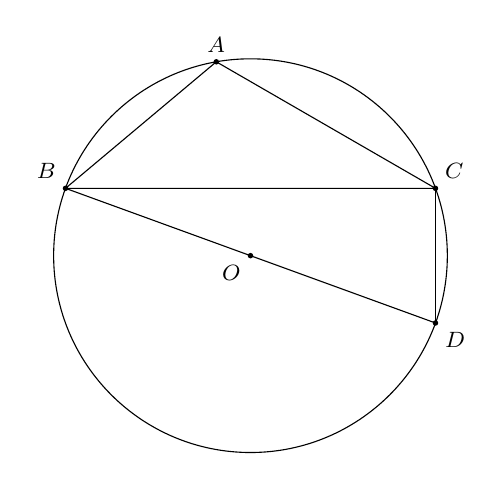
\begin{tikzpicture}[scale=1, font=\footnotesize, line join=round, line cap=round, >=stealth]
				% Vẽ đường tròn tâm O bán kính 3
				\draw (0,0) circle (2.5);
				\fill (0,0) circle (1pt) node[below left] {$O$};
				
				% Tọa độ các điểm
				\coordinate (B) at ({2.5*cos(160)},{2.5*sin(160)});
				\coordinate (C) at ({2.5*cos(20)},{2.5*sin(20)});
				\coordinate (D) at ({2.5*cos(340)},{2.5*sin(340)});  % Đối xứng B qua O
				\coordinate (A) at ({2.5*cos(100)},{2.5*sin(100)});  % A trên cung nhỏ BC, gần B
				
				% Vẽ tam giác ABC
				\draw (A) -- (B) -- (C) -- cycle;
				
				% Vẽ đường kính BD và đoạn CD
				\draw (B) -- (D);
				\draw (C) -- (D);
				
				% Gán nhãn các điểm
				\fill (A) circle (1pt) node[above] {$A$};
				\fill (B) circle (1pt) node[above left] {$B$};
				\fill (C) circle (1pt) node[above right] {$C$};
				\fill (D) circle (1pt) node[below right] {$D$};
			\end{tikzpicture}
		}
	}		
\end{bt}

\begin{bt}%[Dự án EX-9-Đề Cương Toán 9]%[NGOCTRUNG]%[9H3C2-2]
	\immini{
		Một chiếc đĩa cổ bị vỡ, người ta xác định chiếc đĩa có dạng hình tròn tâm $O$. Trên mảnh vỡ được tìm thấy, người ta chọn $3$ điểm $A$, $B$, $C$ thỏa $BC=10$ cm và $\widehat{BAC}=120^{\circ}$. Tính bán kính chiếc đĩa. (\textit{kết quả làm tròn đến hàng phần mười}).
	}{
		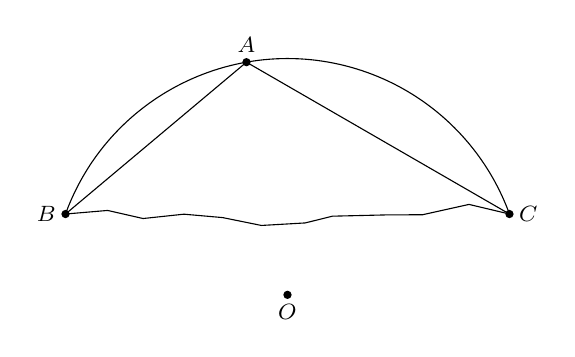
\begin{tikzpicture}[scale=1, font=\footnotesize, line join=round, line cap=round, >=stealth]
			% Tâm và bán kính
			\coordinate (O) at (0,0);
			\def\r{3}
			
			% Các điểm trên đường tròn
			\coordinate (B) at ({\r*cos(160)},{\r*sin(160)});
			\coordinate (C) at ({\r*cos(20)},{\r*sin(20)});
			\coordinate (A) at ({\r*cos(100)},{\r*sin(100)});
			
			% Vẽ cung nhỏ BC nét liền
			\draw (B) arc[start angle=160, end angle=20, radius=\r];
			
			% Vẽ đường gợn sóng không đều thay cho dây BC
			\draw[decorate, 
			decoration={random steps,segment length=5mm,amplitude=1.5mm}] (B) -- (C);
			
			% Vẽ các đoạn AB và AC
			\draw (A) -- (B);
			\draw (A) -- (C);
			
			% Vẽ điểm O
			\fill (O) circle (1.5pt) node[below] {$O$};
			
			% Gán nhãn các điểm
			\fill (B) circle (1.5pt) node[left] {$B$};
			\fill (C) circle (1.5pt) node[right] {$C$};
			\fill (A) circle (1.5pt) node[above] {$A$};
		\end{tikzpicture}
	}
	\loigiai{
		Vẽ $BD$ là đường kính của $(O)$.\\
		Xét tứ giác $ABDC$ có bốn đỉnh $A$, $B$, $D$, $C$ đều thuộc $(O)$ nên từ giác $ABDC$ nội tiếp.
		\immini{
			Do đó $\widehat{BDC}+\widehat{BAC}=180^\circ$ suy ra $\widehat{BDC}=180^\circ-\widehat{BAC}$.\\
			Ta có $\widehat{BCD}=90^{\circ}$ (góc nội tiếp chắn nửa $(O)$) nên $\triangle DBC$ vuông tại $C$.\\
			Xét $\triangle DBC$ vuông tại $C$, ta có
			\allowdisplaybreaks
			\begin{eqnarray*}
				\sin \widehat{BDC} &=& \dfrac{BC}{BD}\\
				\sin\left(180^\circ - \widehat{BAC}\right) &=& \dfrac{BC}{2R}\\
				\dfrac{BC}{\sin\left(180^\circ - \widehat{BAC}\right)} &=& 2R.
			\end{eqnarray*}
		}{
			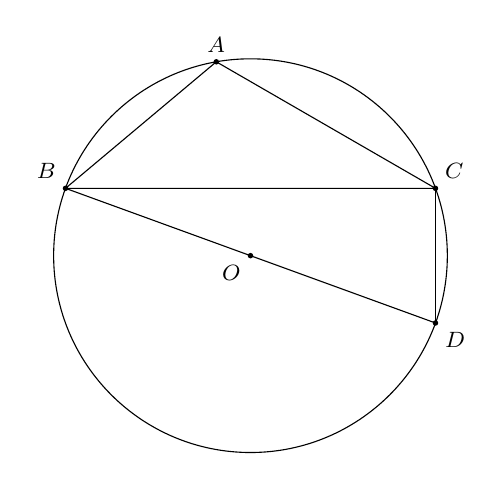
\begin{tikzpicture}[scale=1, font=\footnotesize, line join=round, line cap=round, >=stealth]
				% Vẽ đường tròn tâm O bán kính 3
				\draw (0,0) circle (2.5);
				\fill (0,0) circle (1pt) node[below left] {$O$};
				
				% Tọa độ các điểm
				\coordinate (B) at ({2.5*cos(160)},{2.5*sin(160)});
				\coordinate (C) at ({2.5*cos(20)},{2.5*sin(20)});
				\coordinate (D) at ({2.5*cos(340)},{2.5*sin(340)});  % Đối xứng B qua O
				\coordinate (A) at ({2.5*cos(100)},{2.5*sin(100)});  % A trên cung nhỏ BC, gần B
				
				% Vẽ tam giác ABC
				\draw (A) -- (B) -- (C) -- cycle;
				
				% Vẽ đường kính BD và đoạn CD
				\draw (B) -- (D);
				\draw (C) -- (D);
				
				% Gán nhãn các điểm
				\fill (A) circle (1pt) node[above] {$A$};
				\fill (B) circle (1pt) node[above left] {$B$};
				\fill (C) circle (1pt) node[above right] {$C$};
				\fill (D) circle (1pt) node[below right] {$D$};
			\end{tikzpicture}
		}
		Suy ra $R=\dfrac{BC}{2\sin\left(180^\circ - \widehat{BAC}\right)}=\dfrac{10}{2\sin 60^{\circ}}=\dfrac{10\sqrt{3}}{3}\approx 5{,}8$.
	}	
\end{bt}

\begin{bt}%[SGK CTST Toán 9]%[9H3H2-3]
	Xác định tâm và tính bán kính đường tròn ngoại tiếp hình chữ nhật $ABCD$ trong các trường hợp sau
	\begin{multicols}{2}
		\begin{enumerate}
			\item $AB=6$ cm, $BC=8$ cm.
			\item $AC=9$ cm.
		\end{enumerate}
	\end{multicols}
	\loigiai{
		\begin{enumerate}
			\item Xét $\triangle ABC$ vuông tại $B$, áp dụng định lí Pythagore, ta có 
			$$AC=\sqrt{AB^2+BC^2}=10 \text{ (cm).}$$
			Gọi $I$ là giao điểm của hai đường chéo trong hình chữ nhật $ABCD$.\\
			Suy ra đường tròn ngoại tiếp hình chữ nhật $ABCD$ có tâm $I$ và bán kính $R=\dfrac{AC}{2}=5$ (cm).
			\item Gọi $I$ là giao điểm của hai đường chéo trong hình chữ nhật $ABCD$.\\
			Suy ra đường tròn ngoại tiếp hình chữ nhật $ABCD$ có tâm $I$ và bán kính $R=\dfrac{AC}{2}=\dfrac{9}{2} = 4{,}5$ (cm).
		\end{enumerate}
	}
\end{bt}

\begin{bt}%[SGK CKP Toán 9]%[Dự án EX-9-Đề Cương Toán 9]%[NGOCTRUNG]%[9H3H2-3]
	Xác định tâm và bán kính của đường tròn ngoại tiếp hình chữ nhật $ABCD$ có $AB=12$ cm và $BC=5$ cm.
	\loigiai{
		\immini{
			Gọi $O$ là giao điểm của hai đường chéo $AC$ và $BD$. Khi đó, đường tròn ngoại tiếp hình chữ nhật $ABCD$ có tâm là $O$ và bán kính $R=\dfrac{1}{2}AC$.\\
			Xét $\triangle ABC$ vuông tại $B$, áp dụng định lí Pythagore, ta có
			$$AC=\sqrt{AB^2+BC^2}=\sqrt{5^2+12^2}=13\text{ (cm).}$$
			Do đó $R=\dfrac{1}{2}AC=\dfrac{1}{2}\cdot 13 = 6{,}5$ (cm).
		}{
			\begin{tikzpicture}[scale=1, font=\footnotesize, line join=round, line cap=round, >=stealth]
				\def\r{2.2}
				\path (155:\r) coordinate (A) 
				(-155:\r) coordinate (D)
				(-25:\r) coordinate (C)
				(25:\r) coordinate (B)
				(intersection of A--C and B--D) coordinate (O);
				\draw [thick] 	(A)--(B) node[midway, above, sloped]{$12$ cm}--(C) node[midway, below, sloped]{$5$ cm}--(D)--cycle
				(A)--(C) (B)--(D)
				(O) circle (\r);
				\foreach \x/\g in {A/120,B/60,C/-60,D/-120,O/-90} \fill[black] (\x) circle (1pt)($(\g:5mm)+(\x)$) node {$\x$};
			\end{tikzpicture}
		}
	}
\end{bt}

\begin{bt}%[SGK CD Toán 9]%[Dự án EX-9-Đề Cương Toán 9]%[NGOCTRUNG]%[9H3H2-3]
	\immini{
		Quan sát khung sắt ở hình bên, bạn Nam thấy hình vuông $ABCD$ 
		nội tiếp đường tròn. Bạn Nam đo được độ dài cạnh của hình vuông đó là $2$ dm. Hỏi chu vi của vòng sắt ứng với đường tròn ngoại tiếp hình vuông đó bằng bao nhiêu decimét (\textit{làm tròn kết quả đến hàng phần mười})?}
	{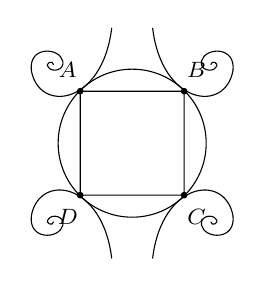
\begin{tikzpicture}[scale=1,font=\footnotesize, line join=round, line cap=round, >=stealth]	
			\tikzset{netcong/.pic={
					\draw
					(5.2,0) .. controls (4.6,4.9) and (0.6,5.4) ..
					(0.1,2.7) .. controls (-0.1,1.1) and (1.9,1.2) ..
					(2.1,2.1) .. controls (2.2,2.7) and (1.4,2.8) ..
					(1.2,2.5) .. controls (0.9,2.2) and (1.5,2) ..
					(1.5,2.3);}}
			\tikzset{hinhve/.pic={
					\path (-.2,.2) pic[scale=.2]{netcong};
					\path (12.8,.2) pic[scale=.2,xscale=-1]{netcong};
					\path (12.8,14.8) pic[scale=-.2]{netcong};
					\path (-.2,14.8) pic[scale=-.2,xscale=-1]{netcong};	
					\draw(6.3,7.5)circle(4.7)
					(3,4.2) coordinate(D)--++(6.6,0)coordinate(C)--++(0,6.6)coordinate(B)--++(-6.6,0)coordinate(A)--cycle ;	}}
			\path (0,0) pic[scale=.2]{hinhve};
			\foreach \d/\g in {A/120,B/60, C/-60, D/-120}	
			\path[draw,fill=black] (\d) circle(1pt) + (\g:9pt) node {$\d$};
	\end{tikzpicture}}
	\loigiai{
		Vì độ dài cạnh của hình vuông $ABCD$ là $2$ dm nên bán kính 
		của đường tròn ngoại tiếp hình vuông đó là $\dfrac{2 
			\sqrt{2}}{2}=\sqrt{2}$ (dm).\\
		Vậy chu vi của vòng sắt ứng với đường tròn ngoại tiếp hình 
		vuông đó là $2 \sqrt{2} \pi \approx 8{,}9$ (dm).
	}
\end{bt}

\begin{bt}%[SGK CD Toán 9]%[Dự án EX-9-Đề Cương Toán 9]%[NGOCTRUNG]%[9H3H2-4] 
	\immini{Mặt trên của tấm đệm có dạng hình tròn  gợi nên 
		hình ảnh đường tròn ngoại tiếp hình chữ nhật. Biết hình chữ nhật đó có chiều rộng, chiều dài lần lượt là $3$ dm, $5$ dm. Tính độ dài đường kính mặt trên của tấm đệm, từ đó tính diện tích mặt trên của tấm đệm (\textit{theo đơn vị dm$^2$ và làm tròn kết quả đến hàng phần trăm}).}
	{\begin{tikzpicture}[scale=0.8, font=\footnotesize, line 
			join=round, 
			line 
			cap=round, >=stealth]
			\def\r{3}
			\def\gocA{110}
			\path (0,0) coordinate (O)
			(10:\r) coordinate (A)
			(70:\r) coordinate (B)
			($(A)!2!(O)$) coordinate (C)
			($(B)!2!(O)$) coordinate (D)
			(-90:\r*1.25) coordinate (x)
			;
			\draw [fill=orange!30!white] (O) circle (\r) ;
			\draw [blue] (A)--(B)--(C)--(D)--cycle ;
	\end{tikzpicture}}
	\loigiai{
		\immini{
			Hình chữ nhật $ABCD$ nội tiếp đường tròn $(O)$ nên đường chéo hình chữ nhật cũng là đường kính của đường tròn $(O)$.\\
			Ta có $\widehat{ABC}=90^\circ$ (góc nội tiếp chắn nửa đường tròn).\\
			Xét $\triangle ABC$ vuông tại $B$, áp dụng định lí Pythagore, ta có
			\allowdisplaybreaks
			\begin{eqnarray*}
				AC^2&=&AB^2+BC^2\\
				AC^2&=&3^2+5^2\\
				AC^2&=&34\\
				AC&=&\sqrt{34} \text{ (dm).}
			\end{eqnarray*}
		}{
			\begin{tikzpicture}[scale=0.8, font=\footnotesize, line join=round, line cap=round, >=stealth]
				\def\r{3}
				\def\gocA{110}
				\path (0,0) coordinate (O)
				(10:\r) coordinate (A)
				(70:\r) coordinate (B)
				($(A)!2!(O)$) coordinate (C)
				($(B)!2!(O)$) coordinate (D)
				;
				\draw [fill=orange!30!white] (O) circle (\r) ;
				\draw [blue] (A)--(B)--(C)--(D)--cycle (A)--(C);
				
				% Nhãn các điểm
				\foreach \d/\g in {A/0, B/90, C/180, O/-90, D/-90}
				\draw (\d) circle (1pt) node[shift={(\g:9pt)}] {$\d$};
				\draw pic [draw, angle radius=2mm] {right angle=A--B--C};
			\end{tikzpicture}
		}
		Độ dài đường kính mặt bên của tấm đệm là 
		$AC=\sqrt{34}\approx5{,}83$ (dm).\\
		Diện tích mặt trên của tấm đệm là
		$S=\pi\cdot\left(\dfrac{\sqrt{34}}{2}\right)^2=\dfrac{17\pi}{2}\approx 26{,}70$ (dm$^2$).
	}
\end{bt}

\begin{bt}%[SGK CTST Toán 9]%[9H3H2-3]
	Cho hình vuông $MNPQ$ nội tiếp đường tròn bán kính $R$. Tính độ dài cạnh và đường chéo của hình vuông theo $R$.
	\loigiai{
		\immini{
			Gọi $I$ là giao điểm của hai đường chéo trong hình vuông $ABCD$.\\
			Khi đó $I$ là trung điểm của $MP$, $NQ$ và $MP\perp NQ$ tại $I$.\\
			Vì $MNPQ$ nội tiếp đường tròn bán kính $R$ nên $MP=NQ=2R$.\\
			Xét $\triangle MNI$ vuông tại $I$, áp dụng định lí Pythagore, ta có
			$$MN=\sqrt{IM^2+IN^2}=R\sqrt{2}.$$
			Vậy cạnh của hình vuông là $R\sqrt{2}$ và đường chéo của hình vuông là $2R$.
		}{
			\begin{tikzpicture}[>=stealth,line join=round,line cap=round,font=\footnotesize,scale=1]
				\path
				(0,0) coordinate (I)
				($(I) + (45:1.9)$) coordinate (N)
				($(I) + (135:1.9)$) coordinate (M)
				($(I) + (225:1.9)$) coordinate (Q)
				($(I) + (315:1.9)$) coordinate (P)
				;
				\draw (I) circle (1.9 cm);
				\draw (M)--(N)--(P)--(Q)--cycle (M)--(P) (Q)--(N);
				\foreach \x/\g in {I/180,N/45,M/135,Q/-135,P/-45} \fill[black] (\x) circle (1pt)+(\g:3mm) node{$\x$};
			\end{tikzpicture}
		}
	}
\end{bt}

\begin{bt}%[SGK CTST Toán 9]%[Dự án EX-9-Đề Cương Toán 9]%[NGOCTRUNG]%[9H3H2-4]
	\immini{
		Một người muốn thiết kế một bảng hiệu gồm một hình vuông nội tiếp một đường tròn có bán kính $R=3$ cm. Tính diện tích hình vuông đó.
	}{
		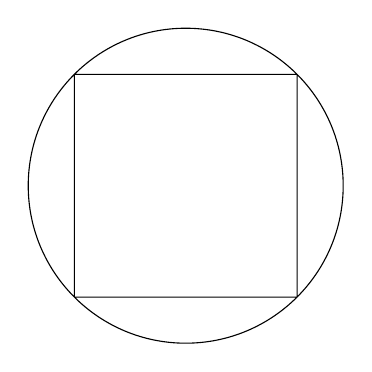
\begin{tikzpicture}[>=stealth,font=\footnotesize,line join=round, line cap=round, scale=1]
			\def\r{2}
			\path (45:\r) coordinate (A) 
			(135:\r) coordinate (B)
			(225:\r) coordinate (C)
			(315:\r) coordinate (D)
			(intersection of A--C and B--D) coordinate (O);
			\draw (A)--(B)--(C)--(D)--cycle
			(O) circle (\r);
			%\foreach \x/\g in {A/120,B/60,C/-60,D/-120,O/-90} \fill[black] (\x) circle (1pt)($(\g:5mm)+(\x)$) node {$\x$};
		\end{tikzpicture}
	}
	\loigiai{
		Đường tròn ngoại tiếp hình vuông có tâm là tâm của hình vuông và đường kính là đường chéo hình vuông.\\
		Do đó, độ dài đường chéo hình vuông là $2R=6$ (cm).\\
		Diện tích của hình vuông đó $S=6^2=36$ (cm$^2$).
	}	
\end{bt}

\begin{bt}%[Dự án EX-9-Đề Cương Toán 9]%[NGOCTRUNG]%[9H3H2-3]
	Cho hình thoi $ABCD$ có các cạnh bằng $3$ cm. Gọi $M$, $N$, $P$, $Q$ lần lượt là trung điểm của $AB$, $BC$, $CA$, $AD$. Chứng tỏ tứ giác $MNPQ$ là hình chữ nhật và tìm bán kính đường tròn ngoại tiếp của tứ giác đó.
	\loigiai{
		\immini{
			Gọi $O$ là giao điểm của $AC$ và $BD$.\\
			Ta có $MN$ là đường trung bình của $\triangle ABC$ nên $MN\parallel AC$ và $MN=\dfrac{1}{2}AC=OA$.\\
			Tương tự, $PQ\parallel AC$ và $PQ=\dfrac{1}{2}AC=OA$.\\
			Suy ra tứ giác $MNPQ$ là hình bình hành.\\
			Mặt khác, ta có $NP$ là đường trung bình của $\triangle ABC$ nên $NP\parallel BD$.\\
			Do đó $MN\parallel AC$, $NP\parallel BD$ và $AC\perp BD$ nên $MN\perp NP$.\\
			Suy ra tứ giác $MNPQ$ là hình chữ nhật.
		}{
			\begin{tikzpicture}[>=stealth,font=\footnotesize,line join=round, line cap=round, scale=1]
				\coordinate (A) at (-3,0);
				\coordinate (C) at (3,0);
				\coordinate (B) at (0,2);
				\coordinate (D) at ($(A)+(C)-(B)$);
				\coordinate (M) at ($(A)!1/2!(B)$);
				\coordinate (N) at ($(B)!1/2!(C)$);
				\coordinate (P) at ($(C)!1/2!(D)$);
				\coordinate (Q) at ($(D)!1/2!(A)$);
				\coordinate (O) at ($(A)!1/2!(C)$);
				\draw(A)--(B)--(C)--(D)--(A)(M)--(N)--(P)--(Q)--(M)(A)--(C)(B)--(D);
				\foreach \p/\g in {A/90,B/90,C/0,D/-90, M/180, N/0, P/-90, Q/-90, O/45}\draw[fill=black] (\p) circle (1pt)node[shift={(\g:.3)},scale=1]{$\p$};
			\end{tikzpicture}
		}
		Bán kính đường tròn ngoại tiếp tứ giác $MNPQ$ là
		$$R=\dfrac{MP}2=\dfrac{\sqrt{MN^2+NP^2}}{2}=\dfrac{\sqrt{OA^2+OB^2}}{2}=\dfrac{AB}{2}=\dfrac{3}{2} = 1{,}5 \text{ (cm).}$$
	}
\end{bt}

